\chapter{Fundamentos teóricos}
\label{estado}
En este capítulo se presentarán las principales temáticas relacionadas con el domino del proyecto, con el objetivo de comprenderlo mejor.

\section{Seguridad Informática}
La seguridad informática forma parte de un término más genérico como es la seguridad de la información, y tiene como objetivo prevenir y detectar el uso no autorizado de un sistema informático.

\subsection{Conceptos previos}

\begin{itemize}
    \item \textbf{Atacante}: Sujeto o entidad que pone en riesgo un sistema
    
    \item \textbf{Ataque}: Consiste en cualquier acción hecha por individuos u organizaciones  que roban, alteran o destruyen a un blanco específico.
    \begin{itemize}
        \item \textbf{Ataque pasivo}: Son aquellos que buscan en el sistema sin llegar a modificar el mismo.
        
        \item \textbf{Ataque activo}: Son aquellos que dañan el objetivo atacado o lo modifican a su favor.
        
    \end{itemize}
     
    \item \textbf{Intrusión}: Conjunto de acciones que intentan comprometer la integridad, confidencialidad o disponibilidad de un recurso. Es decir, la intrusión no solo consiste en el acceso no autorizado sino también en la denegación del acceso a otros usuarios o la manipulación de la información.
    
    \item \textbf{Vulnerabilidad~\cite{incibe_amenaza}}: Debilidad o fallo en un sistema de información que pone en riesgo la seguridad de la información permitiendo que un atacante pueda comprometer la integridad, disponibilidad o confidencialidad de la misma.
     
     
    \item \textbf{Amenaza~\cite{incibe_amenaza}}:Acción que aprovecha una vulnerabilidad para atentar contra la seguridad de un sistema de información. Es decir, que podría tener un potencial efecto negativo sobre algún elemento de nuestro sistema.
    
    \item \textbf{Riesgo~\cite{incibe_amenaza}} : El riesgo es la probabilidad de que se produzca un incidente de seguridad, materializándose una amenaza y causando pérdidas o daños.
    
    \item \textbf{Política de Seguridad~\cite{conceptos_rediris}}: Conjunto de requisitos definidos por los responsables de un sistema que indican en términos generales qué está y qué no está permitido en el área de la seguridad durante el uso del sistema.
    
\end{itemize}



\subsection{Objetivos de la seguridad informática}
Los sistemas de información guardan, distribuyen o generan información para usuarios, empresas, procesos, aplicaciones\dots~ y esta información debe garantizar ciertas características para evitar fraudes. La seguridad informática intenta asegurar estas garantías sobre la información~\cite{objetivos_rediris}:

\begin{itemize}
    \item \textbf{Confidencialidad}: Es la capacidad de que solo los usuarios autorizados puedan acceder a nuestros recursos, datos e información. Este es uno de los principales problemas a los que se enfrentan las empresas.    
    \item \textbf{Integridad}: Es la capacidad de asegurar que los datos sean legítimos, es decir, asegurar que los datos recibidos sean los generados inicialmente y que nada, ni nadie ajeno pueda modificar dichos datos.    
    \item \textbf{Disponibilidad}: Esta característica es de las más importantes y asegura que los datos estén accesibles siempre que el usuario, proceso o sistema lo necesite.    
    
    
\end{itemize}


\subsection{Autenticación de usuario}
En el ámbito de la seguridad informática es muy importante demostrar que un usuario o una aplicación es realmente quien dicha persona o aplicación asegura ser. Para esta verificación se pueden usar varias técnicas~\cite{autenticación_rediris}:

\begin{enumerate}
    \item \textbf{Sistemas basados en algo conocido}: Es el modelo de autenticación más básico y consiste en decidir si un usuario dice ser quien es simplemente basándonos en un prueba que a priori solo ese usuario puede saber.
    Esta aproximación es la más barata y también las más vulnerable a todo tipo de ataques.
    
    Las entidades que participan en la autenticación acuerdan una clave, que mantendrán en secreto. Cuando una de las partes necesita autenticarse solo tiene que mostrar la clave secreta que han acordado para poder acceder a los recursos.
    
    \item \textbf{Sistemas basados en algo poseído}: Este modelo de autenticación es más complejo y se puede complementar con otros sistemas como el anterior de una manera fácil, pero también implica un mayor coste. Por lo general, este modelo se caracteriza por el uso de una tarjeta con un chip integrado el cual incorpora la información necesaria para la autenticación del usuario.    
    Este dispositivo fue patentado por \textbf{Roland Moreno} en 1970, y consistía en una tarjeta de plástico con un chip integrado. A día de hoy este tipo de tarjeta está presente en multitud de aplicaciones como tarjeta bancarias, tarjetas de acceso\dots
\item \textbf{Sistemas de autenticación biométrica}: Hoy en día existen otros mecanismos que se basan en las cualidades del usuario.    
    Este tipo de sistemas basados en el reconocimiento de cualidades físicas del usuario, utilizan características únicas del individuo para su identificación. El proceso general para este tipo de sistemas es el siguiente:
    \begin{enumerate}[label={\arabic*.}]
        \item Se captura una muestra de los datos del usuario.
        \item Se extraen las características que sean únicas de ese usuario.
        \item Se comparan dichas características con las extraídas en un primer momento.
        \item En base a esa comparación se decide si el usuario es quien dice ser.
    \end{enumerate}
    
    Los sistemas de autenticación biométricos más comunes son:
    \begin{itemize}
        \item \textbf{Verificación de huella dactilar}: La huella de un ser humano es un rasgo de identificación único (salvo alguna excepción), pero los sistemas de autenticación miden ciertas características que se han demostrado únicas en los todos los individuos~\cite{Juan_Vucetich}.
        
        \item \textbf{Verificación de patrones oculares}: Estos modelos de reconocimiento mediante patrones oculares, por lo general miden rasgos en el iris o en la retina. Han demostrado ser los más fiables con una probabilidad de coincidencia cercana a cero. 
        
    \end{itemize}
    
    Otros sistemas de autenticación biométricos basados en el comportamiento humano, como el que se trata en este proyecto, son:
    
    \begin{itemize}
        \item \textbf{Reconocimiento de voz}: El reconocimiento de voz intenta detectar características típicas de la voz del usuario para identificarlo. La técnica aplicada para lograr este fin es parecida a los sistemas de reconocimiento de canciones como \textit{shazam}~\cite{shazam}.
        
        
        \item \textbf{Verificación de escritura}: Estos sistemas intentan verificar la firma manuscrita de una persona. En ella se verifican los patrones y características del trazo realizado.
        
        \item \textbf{Sistemas de reconocimiento de escritura por teclado}~\cite{daniel_garabato}: Este tipo de sistemas intenta caracterizar al usuario a partir de ciertos patrones que se producen cuando escribe con un teclado.
        
        \item \textbf{Sistemas de reconocimiento mediante el uso del ratón}~\cite{jorge_rodriguez}: Intentan caracterizar a los usuarios mediante el estudio de las curvas que se trazan cuando se realizan movimientos con el ratón
        
    \end{itemize}
    
    
    
\end{enumerate}



\section{Características del uso de los sensores}

Los dispositivos móviles actuales vienen equipados con un conjunto de sensores~\cite{sensor_draft} que permiten conocer la aceleración, posición, luminosidad\dots~del dispositivo. En este proyecto se han utilizado dos de estos sensores para extraer los datos.

\subsection{Acelerómetro}
Este sensor~\cite{orientatio_draft} es capaz de medir las aceleraciones en tres ejes espaciales~[Figura~\ref{fig:accelerometer_coordinate_system}]. Es decir, es capaz de medir que el dispositivo se está moviendo y con cuanta intensidad lo está haciendo.

\begin{figure}[h]
    \centering
    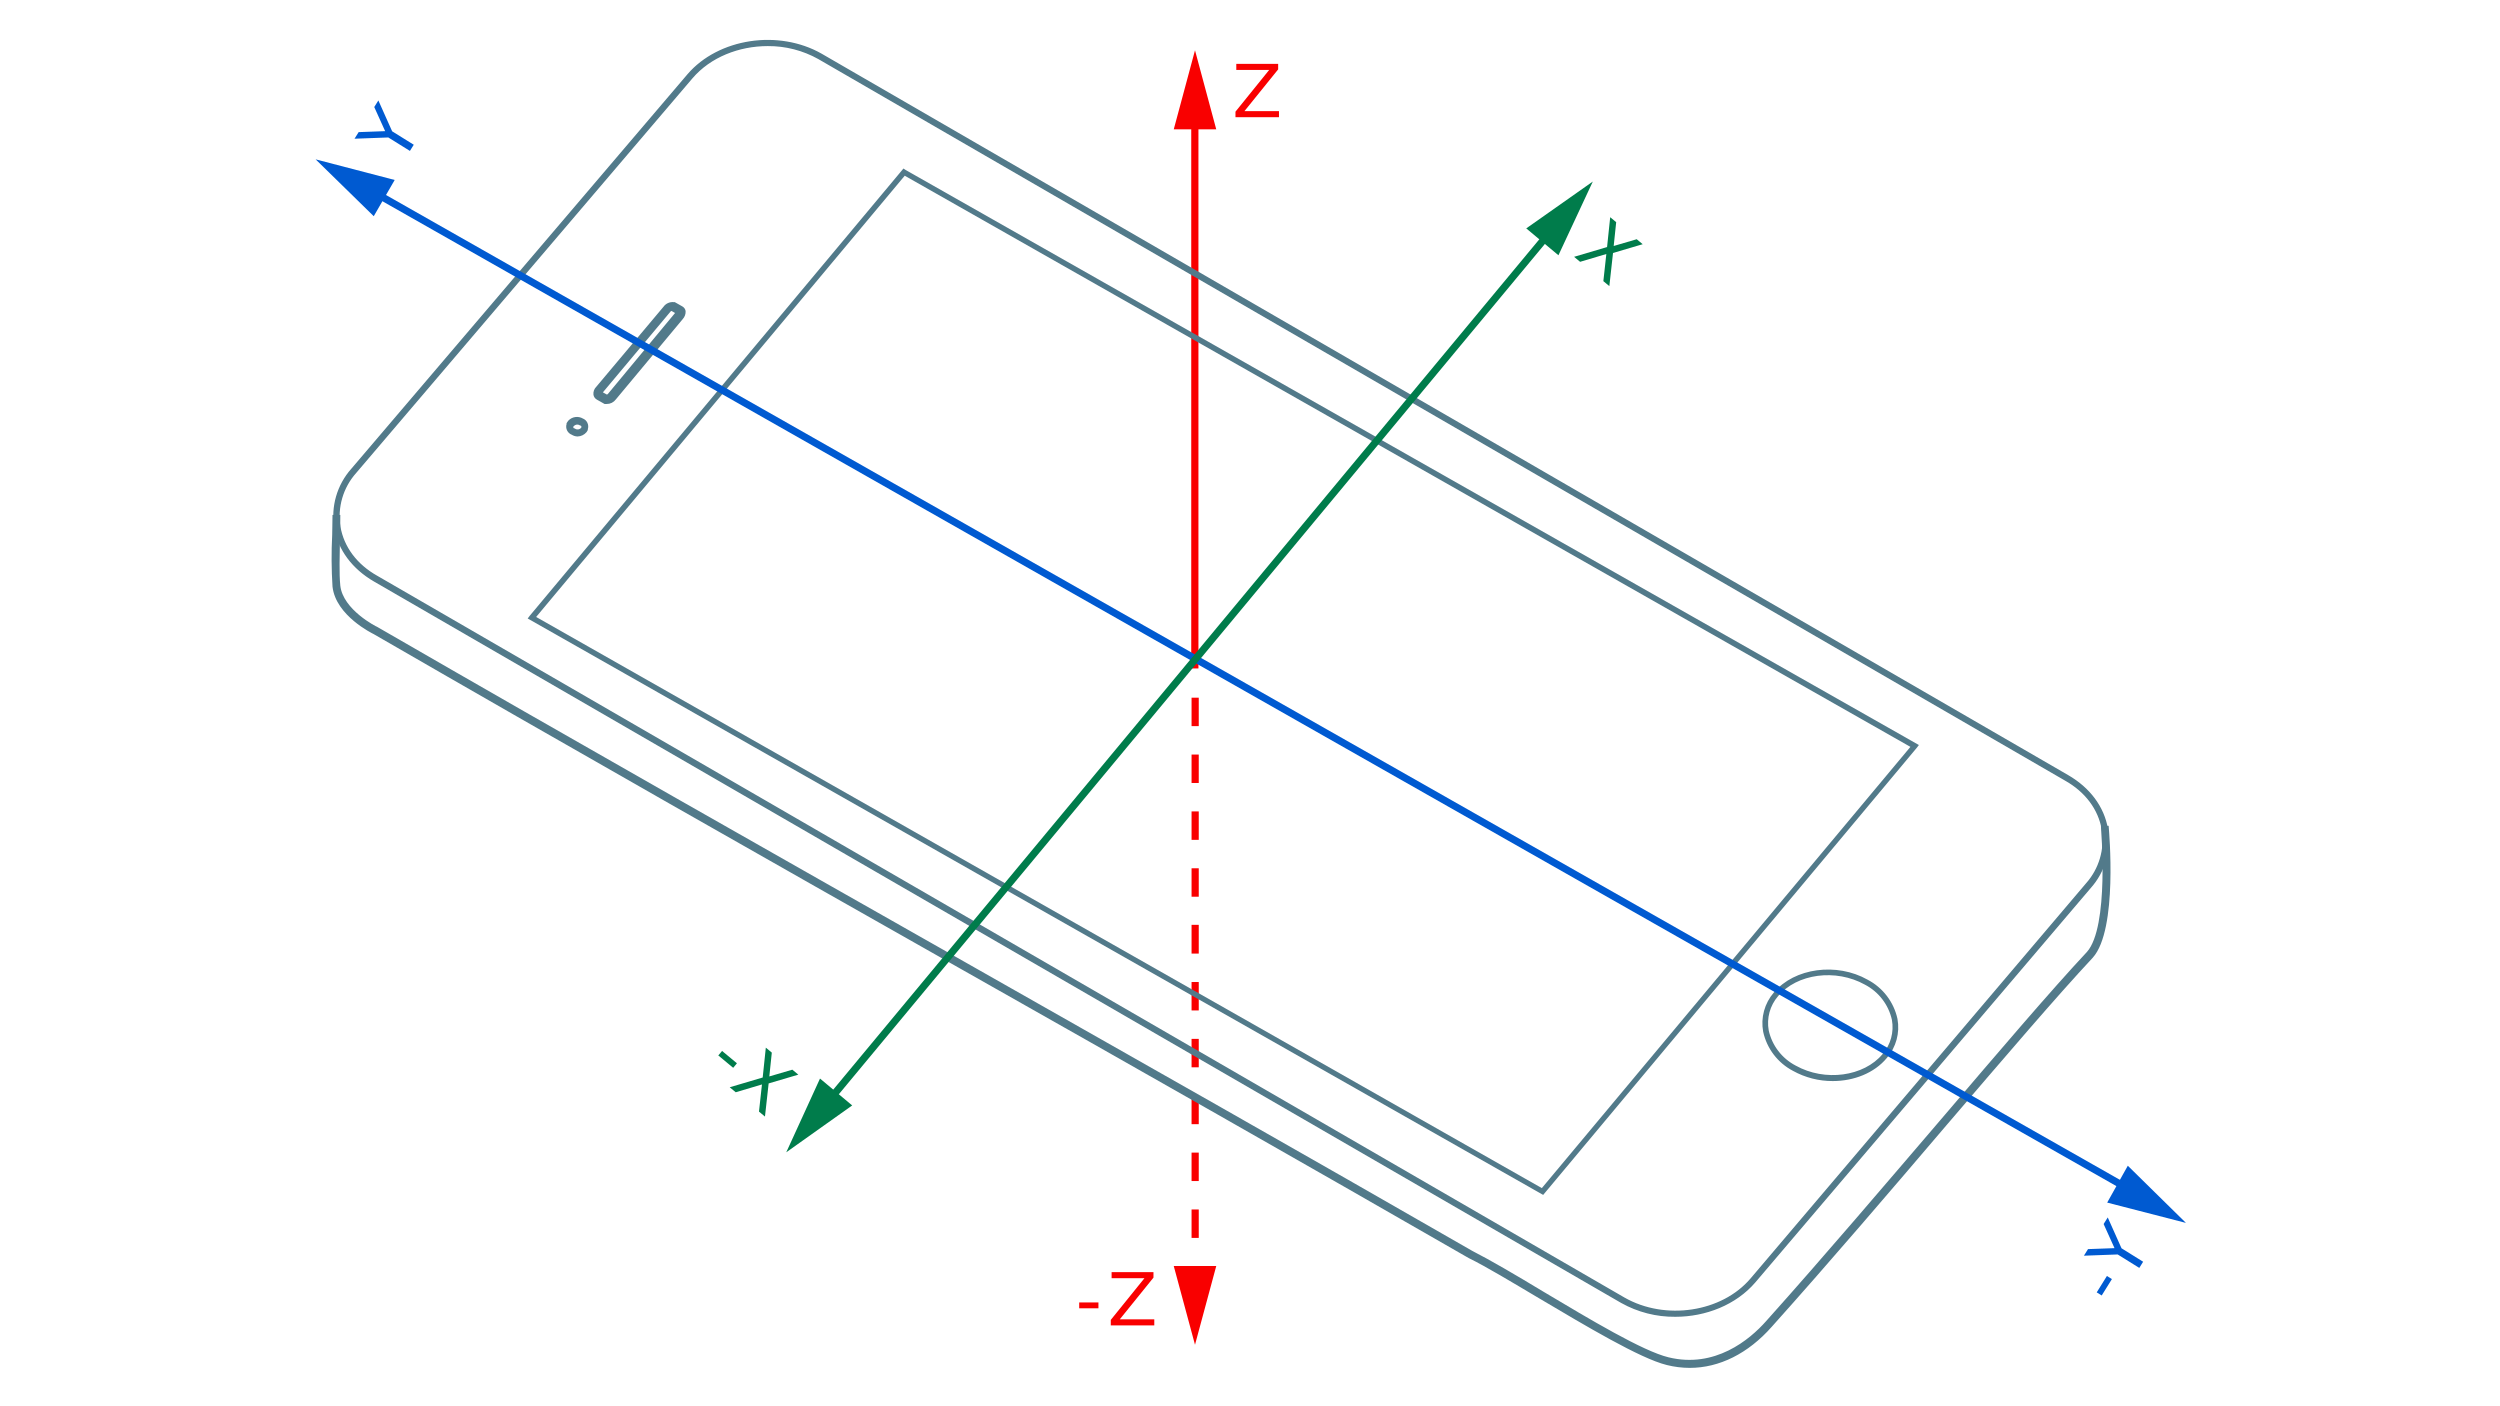
\includegraphics[width=0.6\textwidth, keepaspectratio]{imaxes/accelerometer_coordinate_system.png}
    \caption{Sistema de coordenadas del acelerómetro}
    \label{fig:accelerometer_coordinate_system}
\end{figure}


\subsection{Giroscopio}
Este sensor~\cite{gyroscope_draft} es capaz de medir la rotación del dispositivo en los tres ejes espaciales~[Figura~\ref{fig:gyroscope_sensor_coordinate_system}]. Es decir, nos ofrece la posición exacta en la que se encuentra el dispositivo.
\begin{figure}[h]
    \centering
    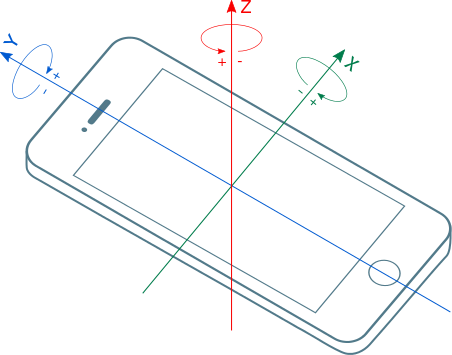
\includegraphics[width=0.5\textwidth, keepaspectratio]{imaxes/gyroscope_sensor_coordinate_system.png}
    \caption{Sistema de coordenadas del giroscopio}
    \label{fig:gyroscope_sensor_coordinate_system}
\end{figure}

\subsection{Extracción de características}
Los sensores mencionados anteriormente ofrecen los datos de un espacio tridimensional. Es decir, nos ofrecen tres valores correspondientes a cada uno de los ejes del espacio.
Debido a que ambos son dependientes de la posición, se ha decidido calcular una cuarta dimensión que no le afecte dicha posición, este nuevo valor es la magnitud que se calcula de la siguiente manera:

\begin{equation}
\texttt{magnitude} = \sqrt{ x^2 + y^2 + z^2}
\end{equation}
Para cada uno de estos cuatro valores obtenidos se han calculado nuevos valores~[Tabla~\ref{tab:sensor_features}] en ventanas de tiempo de cinco segundos. Estos valores, con ventanas de cinco segundos, han sido utilizados en otros estudios~\cite{ehatisham2018continuous} con buenos resultados. 

\begin{table}[H]
    \centering
    \begin{tabular}{l p{0.6\linewidth}}
    \toprule
    Nombre & Descripción \\
    \midrule
        \textbf{Media} &   Es un medida con tendencia al valor central. \\
        \textbf{Desviación estándar} &  Mide cuánto se separan los datos con respecto a la media aritmetica. \\
        \textbf{Varianza} &   Es el valor de la desviación estándar al cuadrado \\
        \textbf{Mínimo} &   Es el valor mínimo del conjunto. \\
        \textbf{Máximo} &   Es el valor máximo del conjunto. \\
        \textbf{Skewness} &   Es una variable que indica la asimetría de la distribución frente a la media. \\
        \textbf{Kurtosis} &   Es una variable que muestra la frecuencia de los datos. \\
    \bottomrule
    \end{tabular}
    \caption{Características de los sensores}
    \label{tab:sensor_features}
\end{table}

\section{Características del uso de la pantalla táctil}
La mayoría de los dispositivos de hoy en día son táctiles y, por lo tanto cuentan con una pantalla que es capaz de generar información sobre la interacción que el usuario realiza. Esta información~\cite{touch_events} extraída se calcula en base a la posición y tiempo entre el primer y último contacto con la pantalla.

A partir de la concatenación de varios de estos eventos en el tiempo, se pueden llegar a extraer otros más complejos como arrastrar, rotar\dots~ Para este proyecto se han capturado los mostrados en la Tabla~\ref{tab:event_type}.

\begin{table}[!h]
    \centering
    \begin{tabular}{l l p{0.6\linewidth}}
    \toprule
    Número de puntos & Nombre & Descripción \\
    \midrule
\multirow{4}{*}{Un sólo punto} & \textbf{Swipe} &   Es el movimiento de deslizamiento. \\
                                  & \textbf{Tap} &  Tocar la pantalla durante un corto periodo de tiempo \\
                                  & \textbf{Press} &  Tocar la pantalla durante un largo periodo de tiempo. \\
                                  & \textbf{Pan} &  Es el movimiento de arrastrar. \\
\midrule
\multirow{2}{*}{Dos puntos}  & \textbf{Pinch} &  Es el movimiento de juntar o separar los dedos para hacer zoom. \\
                                & \textbf{Rotate} &  Es el movimiento de girar los dedos para hacer rotar un objeto. \\
    \bottomrule
    \end{tabular}
    \caption{Tipos de eventos}
    \label{tab:event_type}
\end{table}

Como los eventos \textit{press} son poco frecuentas en cualquier tipo de aplicación se ha decidido descartarlos para el análisis.  Los eventos de \textit{pinch} y \textit{rotate} se han unido en un solo evento, puesto que ambos generan las mismas características. Este nuevo evento generado se ha llamado \textit{multitouch}.
La Tabla~\ref{tab:event_features} muestra las características extraídas para cada tipo de evento, que serán utilizadas para el análisis.


\begin{center}
    \begin{longtable}{l l p{0.6\linewidth}}
    \toprule
    Ev. & Nombre & Descripción \\
    \midrule
\multirow{8}{*}{\rotatebox[origin=c]{90}{Swipe}} & \textbf{duration}       & Duración del evento en milisegundos \\
                       & \textbf{distance}       & Distancia recorrida del evento en píxeles \\
                       & \textbf{velocity}       & Velocidad media del evento en píxeles/milisegundos  \\
                       & \textbf{angle}          & Ángulo creado desde el punto inicial al punto final \\
                       & \textbf{width}          & Ancho del área de pulsación en píxeles \\
                       & \textbf{height}         & Alto del área de pulsación en píxeles \\
                       & \textbf{frame\_index}   & Posición en la pantalla donde ha ocurrido el evento \\
                       & \textbf{direction}      & Dirección del evento \\
\midrule
\multirow{5}{*}{\rotatebox[origin=c]{90}{Tap}}   & \textbf{duration}       & Duración del evento en milisegundos \\
                       & \textbf{distance}       & Distancia recorrida del evento en píxeles \\
                       & \textbf{width}          & Ancho del área de pulsación en píxeles \\
                       & \textbf{height}         & Alto del área de pulsación en píxeles \\     
                       & \textbf{frame\_index}  & Posición en la pantalla donde ha ocurrido el evento \\
\midrule

\multirow{11}{*}{\rotatebox[origin=c]{90}{Pan}}  
& \textbf{duration} & Duración del evento en milisegundos \\
& \textbf{distance} & Distancia recorrida del evento en píxeles \\
& \textbf{velocity} & Velocidad media del evento en píxeles/milisegundos \\
& \textbf{angle} & Ángulo creado desde el punto inicial al punto final \\
& \textbf{width}              & Ancho del área de pulsación en píxeles \\
& \textbf{height}             & Alto del área de pulsación en píxeles\\ 
& \textbf{angle\_total}       & Suma de los ángulos realizados a lo largo del recorrido.\\ 
& \textbf{velocity\_y}        & Suma total de las velocidades a lo largo del recorrido, sobre el eje Y. \\
& \textbf{velocity\_x}        & Suma total de las velocidades a lo largo del recorrido, sobre el eje X. \\ 
& \textbf{avg\_velocity\_x}   & Velocidad media en el eje X \\ 
& \textbf{avg\_velocity\_y}   & Velocidad media en el eje Y \\ 
\midrule
\multirow{15}{*}{\rotatebox[origin=c]{90}{Multitouch}}  & \textbf{area}            & Área cubierta del evento, tomando como vértices los puntos mínimos y máximos de los dedos \\ 
                              & \textbf{abfs}            & Ángulo entre los dos primeros puntos\\ 
                              & \textbf{abfe}            & Ángulo entre los dos últimos puntos\\ 
                              & \textbf{rbfs}            & Distancia entre los dos primeros puntos eje y\\ 
                              & \textbf{rbfe}            & Distancia entre los dos primeros puntos eje x\\ 
                              & \textbf{df\_up}          & Distancia entre del dedo superior eje x\\ 
                              & \textbf{df\_dow}         & Distancia entre del dedo inferior eje x\\ 
                              & \textbf{avg\_width\_0}   & Ancho del área de pulsación en píxeles\\ 
                              & \textbf{avg\_width\_1}   & Ancho del área de pulsación en píxeles\\ 
                              & \textbf{avg\_height\_0}  & Alto del área de pulsación en píxeles\\ 
                              & \textbf{avg\_height\_1}  & Alto del área de pulsación en píxeles\\ 
                              & \textbf{velocity\_dow}   & Velocidad media del dedo inferior\\ 
                              & \textbf{velocity\_up}    & Velocidad media del dedo superior\\ 
                              & \textbf{duration}        & Duración del evento en milisegundos\\ 
                              & \textbf{direction}      & Dirección del evento \\

    \bottomrule
    \caption{Características por tipo de evento}
    \label{tab:event_features}
    \end{longtable}
\end{center}



\section{Evaluación del rendimiento}
\label{sec:metrics}

Para analizar los resultados obtenidos y comprobar la fiabilidad de los algoritmos usados, necesitamos emplear unas métricas que evalúen su rendimiento y permitan comparar diferentes aproximaciones.

Al ser este un problema de clasificación binaria (usuarios legítimos, usuarios no legítimos) se ha utilizado la matriz de confusión~[Figura~\ref{fig:matrix_conf}], la cual categoriza los datos en cuatro grupos:


\begin{itemize}
    \item \textbf{Verdaderos Negativos (TN)}: Es la cantidad de negativos que fueron clasificados correctamente como negativos.
    
    \item \textbf{Falsos Positivos (FP)}: Es la cantidad de negativos que fueron clasificados incorrectamente como positivos.
    
    \item \textbf{Falsos Negativos (FN)}: Es la cantidad de negativos que fueron clasificados incorrectamente como negativos.
    
    \item \textbf{Verdaderos Positivos (TP)}: Es la cantidad de positivos que fueron clasificados correctamente como positivos.
\end{itemize}


\begin{figure}[H]
    \centering
    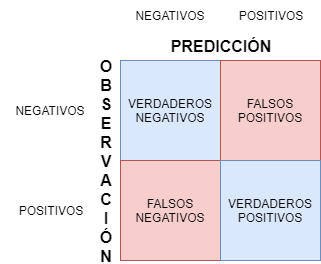
\includegraphics[width=0.5\textwidth, keepaspectratio]{imaxes/matriz_confusion.png}
    \caption{Esquema matriz de confusión}
    \label{fig:matrix_conf}
\end{figure}

A partir de los datos obtenidos de una matriz de confusión, se pueden calcular medidas que permiten obtener una representación analítica de los resultados. Por otra parte, durante el entrenamiento de los algoritmos también se han calculado los tiempos de cómputo.

\begin{itemize}
    \label{list:scores}
    \item\textbf{Recall (RC)}: Es la relación entre las predicciones positivas correctas y el total de observaciones positivas.
        \begin{equation}
            \frac{TP}{TP + FN}
        \end{equation}
    
    \item \textbf{Precision (PS)}: Es la relación entre las predicciones positivas correctas y el total de predicciones positivas.
        \begin{equation}
            \frac{TP}{TP  + FP}
        \end{equation}
    
    \item \textbf{F1}: Es la media armónica de los valores anteriores. 
        \begin{equation}
            \frac{2}{\frac{1}{precision} + \frac{1}{recall}} = 2 * \frac{precision * 
    recall}{precision + recall} = \frac{TP}{TP + \frac{FN + FP}{2}}
        \end{equation}
    
    \item \textbf{Accuracy}: Es la relación entre las predicciones positivas y el total de casos.
        \begin{equation}
            \frac{TP}{TP + FP + FN + TN} 
        \end{equation}
    
    
    \item \textbf{Fit Time}: Tiempo de cómputo que ha tardado en entrenar el algoritmo.
    
    \item \textbf{Score Time}: Tiempo de cómputo que ha tardado en ejecutar la predicción.
\end{itemize}

Para analizar los resultados, se ha favorecido el uso de la métrica \textit{precision} para tratar de minimizar posibles intrusiones.



\section{Inteligencia Artificial}

En 1956, \textbf{Jhon McCarthy}~\cite{jhonmccarthy}, conocido como el padre de la Inteligencia Artificial, acuñó el término Inteligencia Artificial, en adelante \textit{IA}, como la ciencia y la ingeniería de hacer máquinas inteligentes, especialmente programas informáticos inteligentes.

En la \textit{IA} existen dos grupos definidos, fuerte y débil. La  \textit{IA} fuerte es aquella que tiene las mismas características que un humano inteligente. La \textit{IA} débil es aquella que muestra inteligencia en un área en concreto pero carece de la misma en otras.

Para conseguir dotar de inteligencia a una máquina se suele utilizar el aprendizaje máquina o \textit{machine learning}. El aprendizaje máquina, en adelante \textit{ML}, es una de las áreas más extendidas de la \textit{IA}. En 1959, \textbf{Arthur Samuel}~\cite{arhtursamuel} definió \textit{ML} como el campo de estudio que brinda a las computadoras la capacidad de aprender sin estar programado explícitamente.

\subsection{Tipo de aprendizaje}

Dentro del \textit{ML} se pueden distinguir dos tipos de aprendizaje:

\begin{itemize}
    \item \textbf{Aprendizaje supervisado}: Los algoritmos son entrenados en base a un conjunto de datos de los que conocemos su respuesta correcta. De esta manera lo que se intenta es que el algoritmo obtenga la respuesta correcta a partir de las características disponibles.
    
    \begin{itemize}
        \item \textbf{Problemas de regresión}: Son usados para evaluar las relaciones que existen entre las variables y obtener un valor de esa estimación.
        \item \textbf{Problemas de clasificación}: Son utilizados para dividir un conjunto de datos de entrada en distintas clases según sus características.
    \end{itemize}
    
    \item \textbf{Aprendizaje no supervisado}: En este modelo, los datos no contienen una respuesta correcta. Este tipo de aprendizaje intenta buscar ciertos patrones o respuestas, pero no una respuesta concreta.
\end{itemize}

%En este proyecto se ha usado el aprendizaje supervisado para clasificar nuestros datos en función de las características extraídas y de esta manera decidir si un usuario es legítimo o no.

La finalidad de todos estos tipos de aprendizajes es la de generalizar, es decir, que puedan resolver problemas que no han visto. 
Cuando entrenamos modelos computacionales con un conjunto de datos de entrada estamos haciendo que el algoritmo sea capaz de generalizar un concepto para que al consultarle por un nuevo conjunto de datos desconocido este sea capaz de comprenderlo y proporcionarnos un resultado fiable~[Figura~\ref{fig:over-under-fitting}].

Si nuestros datos de entrenamiento son muy pocos o poco representativos nuestra máquina no será capaz de generalizar el conocimiento y estará incurriendo en \textit{underfitting}~[Figura~\ref{fig:over-under-fitting}].

Si sobrentrenamos nuestro modelo lo que ocurrirá es que nuestra máquina sólo se limitará a memorizar los casos particulares que le enseñamos y será incapaz de reconocer nuevos datos de entrada, perdiendo toda capacidad de generalización.



\begin{figure}[h]
    \centering
    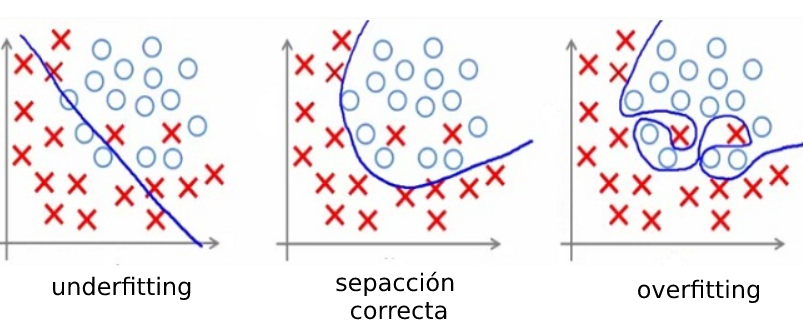
\includegraphics[width=0.7\textwidth, keepaspectratio]{imaxes/overfitting.png}
    \caption{Problemas de entrenamiento}
    \label{fig:over-under-fitting}
\end{figure}


% ======================================================== %

% ======================================================== %

\subsection{Redes Neuronales Artificiales}
Las redes neuronales artificiales~\cite{salas2004redes}, en adelante \textit{RNA}, son un modelo computacional inspirado en la estructura del sistema nervioso de los seres humanos. La unidad elemental de una \textit{RNA} es la neurona artificial [Figura~\ref{fig:neurona}] y generalmente están organizadas en capas. Poseen varias entradas y una salida, que se calcula normalmente realizando una suma ponderada de las entradas con sus pesos~[\ref{eq:perceptron}]. 

\begin{equation} \label{eq:perceptron}
    \displaystyle\sum_{i=1}^{n} w_i x_i + w_0= 
    \begin{cases}
        \geq 0       & \quad y = 1 \\
        <    0       & \quad y = 0
    \end{cases}
\end{equation}

Este resultado es modificado por una función de activación y el valor obtenido se transmite directamente al siguiente elemento. Normalmente para conseguir esta transformación se emplean funciones como la sigmoidal, gaussiana o la tangente hiperbólica:

\begin{itemize}
    \item Función sigmoidal: 
    \begin{equation}
        f(x) = \frac{1}{1 + e^{-x}}
    \end{equation}
    
    \item Función tangente hiperbólica: 
    \begin{equation}
        f(x) = tanh(x)
    \end{equation}
    
    \item Función gaussiana: 
    \begin{equation}
        f(x) = e^{\frac{-x^2}{2}}
    \end{equation}
    
    
\end{itemize}



\begin{figure}[H]
    \centering
    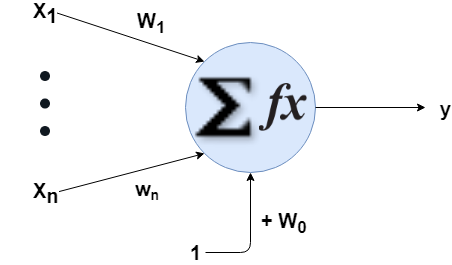
\includegraphics[width=0.7\textwidth, keepaspectratio]{imaxes/neurona.png}
    \caption{Esquema de un neurona artificial}
    \label{fig:neurona}
\end{figure}







% ======================================================== %

% ======================================================== %

\subsection{Perceptrón Multicapa}
\label{sec:mlp}

En 1958, \textbf{Rosenblatt}~\cite{rosenblatt1960perceptron} diseñó y desarrollo el perceptrón. Este modelo implementa el funcionamiento de una sola neurona que es capaz de resolver problemas lineales. En 1969, \textbf{Minsky y Papert} escribieron un libro~\cite{minsky2017perceptrons} donde demostraron que un solo perceptrón era incapaz de aprender la función exclusiva (XOR), es decir, problemas cuya resolución no es lineal. En este mismo libro se expone un nuevo paradigma de \textit{RNA} llamado perceptrón multicapa  también conocido como \textit{MLP} por sus siglas en inglés (\textit{Multi-Layer Perceptron}). Este modelo es una combinación de varios perceptrones, que permiten aproximar cualquier problema, aunque no sea lineal. Éste se caracteriza por tener sus neuronas agrupadas en capas de diferentes niveles, por lo general tres~[Figura~\ref{fig:schematic_MLP}]. 

\begin{itemize}
    \item \textbf{Capa de entrada }: Esta capa conecta la red con el exterior, cada neurona se corresponde con cada una de las variables de entrada a la red.
    
    \item \textbf{Capas ocultas }: Es un conjunto de capas que cuyas entradas son las salidas de la capa anterior y cuya salida pasan a la capa sucesora.
    
    \item \textbf{Capa de salida }: Conecta las capas ocultas con la salida de la red que proporciona los resultados.
\end{itemize}

Además, sus conexiones están dirigidas hacia adelante, es decir, las neuronas de una capa se conectan con las neuronas de la siguiente capa y generalmente todas las neuronas de una capa se encuentran enlazadas con las de la siguiente capa.


\begin{figure}[H]
    \centering
    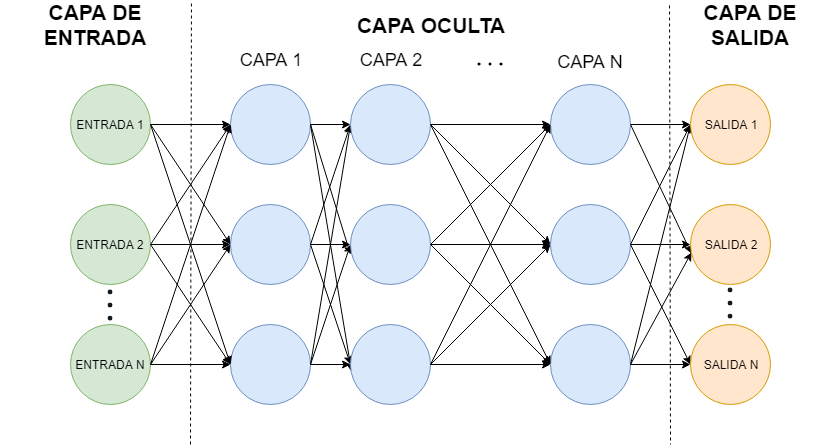
\includegraphics[width=0.9\textwidth, keepaspectratio]{imaxes/schematic_mlp.png}
    \caption{Esquema del MLP}
    \label{fig:schematic_MLP}
\end{figure}

Inicialmente, este planteamiento no se pudo materializar porque no existía un mecanismo que ajustase automáticamente los pesos de la capa oculta. En 1986, \textbf{Rummelhart, Hinton y Wiliams} desarrollan la \textit{Regla Delta Generalizada}~\cite{rumelhart1988learning} para adaptar los pesos propagando los errores hacia atrás. De esta manera se demuestra que el \textit{MLP} es capaz de resolver problemas lineales y no lineales.

En la Figura~\ref{fig:MLP_example} se puede ver el funcionamiento del \textit{MLP}. En ella se muestra el esquema de un \textit{MLP} que contiene una capa de entrada, dos capas ocultas y la salida. 
Cada neurona está representada visualmente con una gráfica que muestra la función aplicada a los datos, por ejemplo, en la capa de entrada, las variables de entrada son dos funciones que dividen los datos en vertical~($X_1$) y horizontal~($X_2$). También se pueden observar la distintas conexiones que existen entre las neuronas e incluso el peso de las conexiones representadas por un color y grosor diferentes.

\begin{figure}[!h]
    \centering
    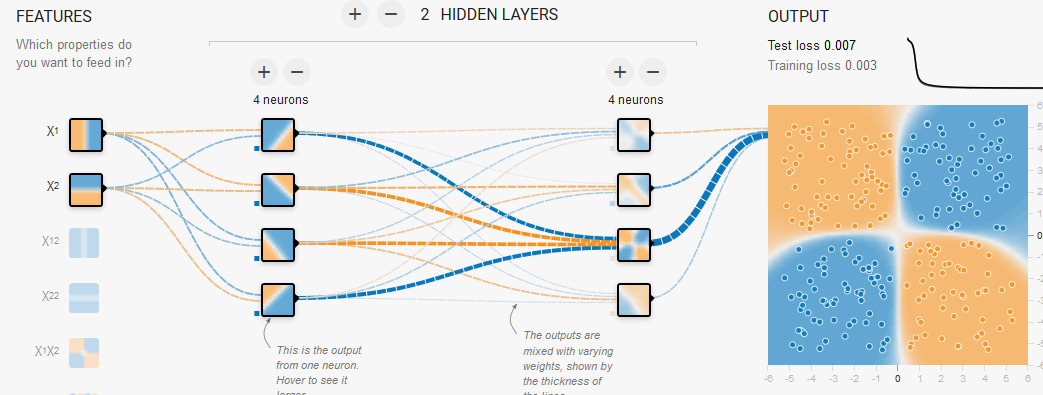
\includegraphics[width=0.9\textwidth, keepaspectratio]{imaxes/MLP_example.png}
    \caption[Ejemplo de una MLP]{Ejemplo de una MLP~\cite{tensorflow}}
    \label{fig:MLP_example}
\end{figure}


Este tipo de arquitectura es muy utilizada debido a su capacidad de aproximación universal. No obstante, requieren un largo proceso de aprendizaje para problemas complejos que requieren de un gran número de variables y una arquitectura compleja.


% ======================================================== %

% ======================================================== %

\subsection{Maquinas de soporte vectorial}
\label{sec:svm}
Las máquinas de soporte vectorial~\cite{berwick2003idiot} también conocidas como \textit{SVMs} de sus siglas en inglés (\textit{Support Vector Machines}), es un conjunto de algoritmos desarrollados por \textbf{Vladimir Vapnik}, capaces de realizar clasificaciones, regresiones e incluso detectar valores atípicos. 


Las \textit{SVMs} generan un hiperplano\footnote{Es un plano de una dimensión inferior al origen, que divide el espacio en dos mitades} para intentar clasificar los datos [Figura~\ref{fig:svm_example}]. En dicho hiperplano se forma una \textit{calle} para separar los datos, donde la línea continua separa el conjunto y las líneas discontinuas indican el margen de error. Las \textit{SVMs} intentan maximizar el margen de error, lo que ocasiona una \textit{calle} más grande y por lo tanto generalizará mejor el problema.

\begin{figure}[h]
    \centering
    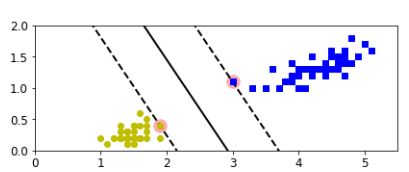
\includegraphics[width=0.7\textwidth, keepaspectratio]{imaxes/svm_exmaple.png}
    \caption{Ejemplo de Clasificación SVM}
     \label{fig:svm_example}
\end{figure}


\subsubsection{Tipos de problemas}

El conjunto de datos utilizados por estos algoritmos suelen ser multidimensionales, por lo tanto, en ciertas ocasiones puede ser complicado separar los datos. En base a esto podemos encontrarnos con dos tipos de escenarios:

\begin{itemize}
    \item \textbf{Lineales~[Figura~\ref{fig:svm_example}] } : La solución de este tipo de problemas genera un hiperplano que es capaz de separar el conjunto de datos perfectamente.
    
    \item \textbf{No lineales}: Son aquellos en los que el conjunto de entrada no es posible separarlos con un hiperplano, pero el hecho de que no sean separables en el espacio original, no significa que no lo sean en un espacio de dimensiones distinto. Para transformar el espacio de entradas a una dimensión diferente se emplean las funciones kernel:
    \begin{itemize}
    \item \textbf{Lineal} : Kernel utilizado cuando pretendemos aproximar nuestra función con una función lineal.
        \begin{equation}
            K(x,y) =  x y + c
        \end{equation}
        donde $c$ es una constante.
    \item \textbf{Polinómica}: Representa la similitud de los vectores en un espacio polinómico distinto al original.
        \begin{equation}
            K(x,y) = (a + xy)^d
        \end{equation}
    donde $d$ es el orden del polinomio y $a$ es una constante.

    \item \textbf{Función de base radial Gaussiana (RBF )~[Figura~\ref{fig:kernel_clf}]}: Genera un nuevo espacio calculando las distancias entre un puntos concreto y el resto de puntos.
    
    \begin{equation}
        K(x,y)=exp(- \frac{||x-y||^2}{2\sigma^2})
    \end{equation}
    
    donde $\sigma$ es la anchura del kernel y $||x-y||$ es la distancia euclídea\footnote{es la distancia entre dos puntos de un espacio euclídeo, la cual se deduce a partir del teorema de Pitágoras.} entre $x$ e $y$ 

    \item \textbf{Función sigmoide}: Aplica la función sigmoide para generar un nuevo espacio de valores.
        \begin{equation}
            K(x,y)=tanh(\alpha x y+ c)   
        \end{equation}
    donde $\alpha$ es la pendiente y $c$ es una constante.
    \end{itemize}
\end{itemize}



\begin{figure}[H]
    \centering
    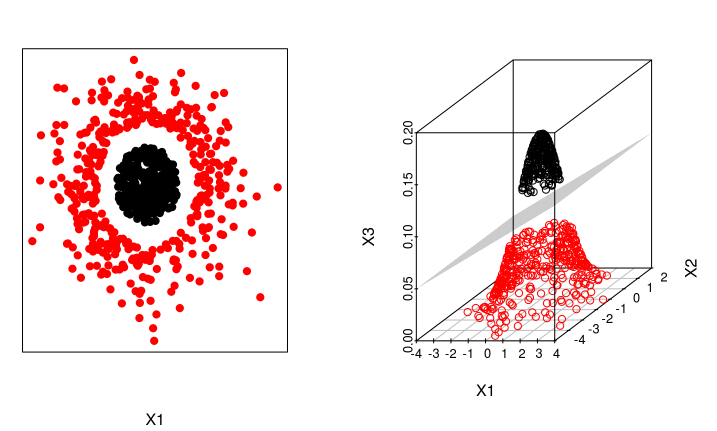
\includegraphics[width=0.7\textwidth, keepaspectratio]{imaxes/svm_exmaple_clf.png}
    \caption[Ejemplo de Clasificación SVM no lineal, usando función gaussiana]{Ejemplo de Clasificación SVM no lineal, usando función gaussiana \cite{joaquin}}
     \label{fig:kernel_clf}
\end{figure}

\subsection{Árboles de Decisión}
\label{sec:decision_tree}
Generan modelos de clasificación o regresión usando árboles como estructuras internas~[Figura~\ref{fig:decisiontree}]. En dicha estructura cada nodo representa una característica del problema, cada rama representa una decisión de esa característica y los nodos hoja contienen el valor de la predicción o clase.

\begin{figure}[h]
    \centering
    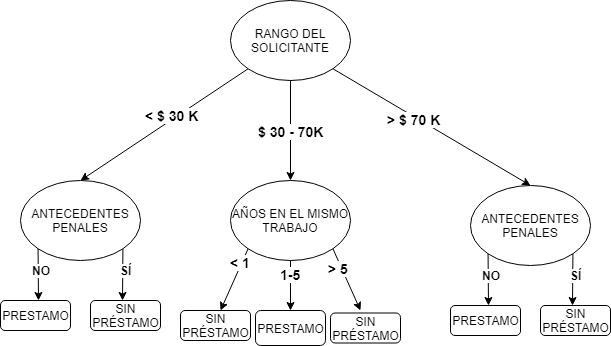
\includegraphics[width=0.7\textwidth, keepaspectratio]{imaxes/decision_tree.png}
    \caption{Árbol de decisión para conceder un préstamo}
    \label{fig:decisiontree}
\end{figure}

\subsection{Regresión Logística}
\label{sec:logistic_regresion}
Es un algoritmo de clasificación usado para asignar un conjunto de valores a dos tipos de clases. 
Para obtener el valor de la predicción utiliza la función sigmoide.

\begin{equation}
    \label{eq:sigmoide}
    S(x) = \frac{1}{1+e^{-x}}
\end{equation}

\subsection{\textit{k-Nearest Neighbours}}
\label{sec:kn}
Es un método que busca en las observaciones más cercanas a la que se está tratando de predecir y clasifica en base a la mayoría de datos que lo rodean~[Figura~\ref{fig:k_n}]. Las técnicas utilizadas para calcular las distancias suelen ser distancia euclidiana, distancia Manhattan\dots

\begin{figure}[!h]
    \centering
    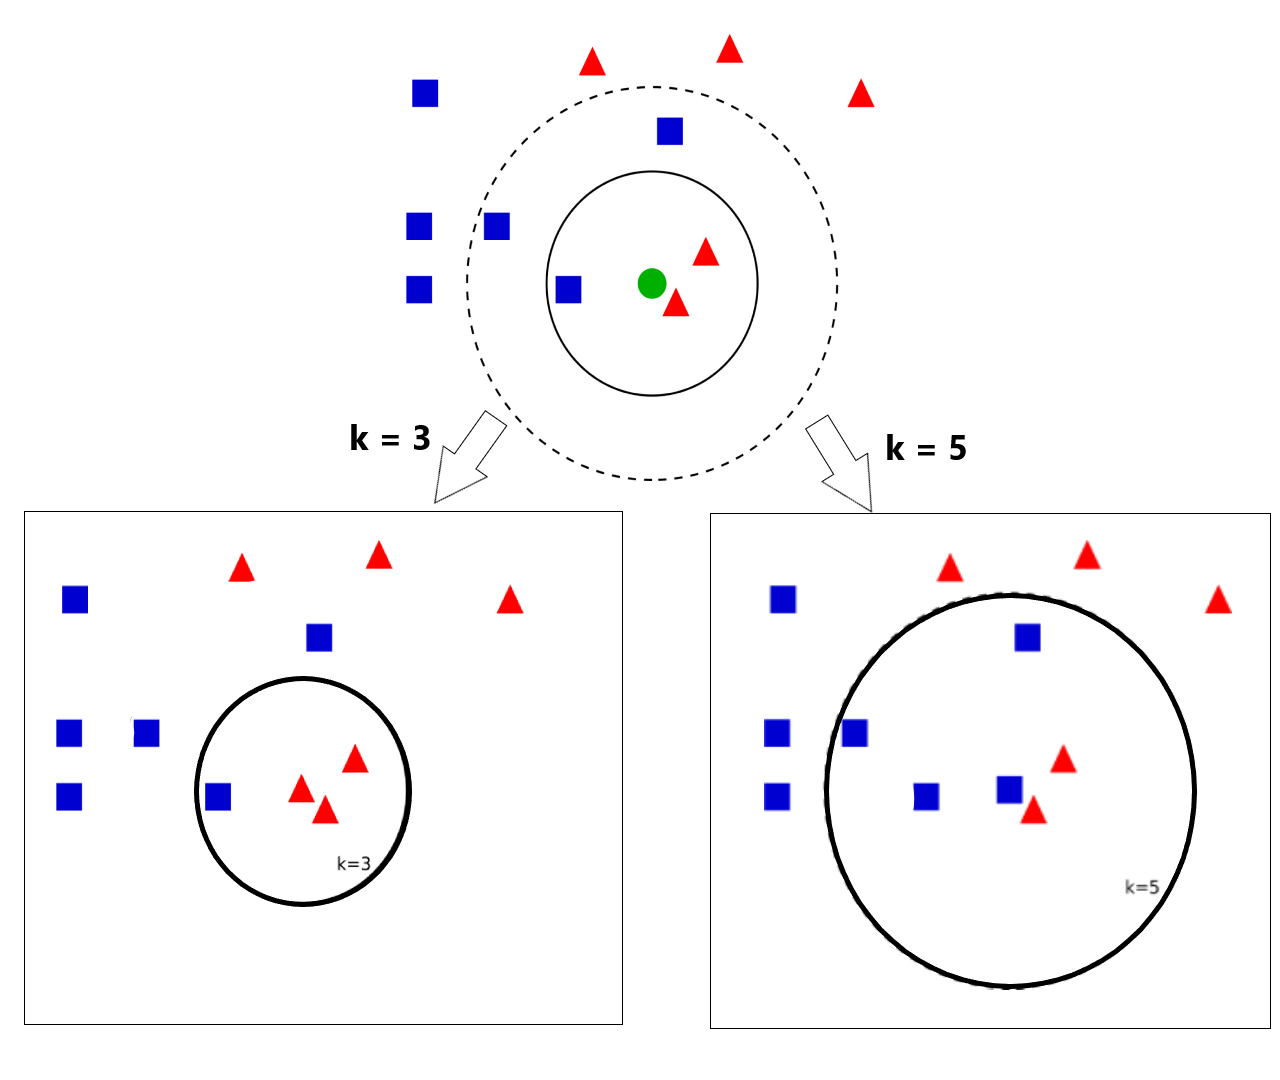
\includegraphics[width=0.7\textwidth, keepaspectratio]{imaxes/KnnClassification.png}
    \caption{Ejemplo de k-Nearest Neighbours}
    \label{fig:k_n}
\end{figure}

\subsection{Métodos Ensambladores}
Los métodos de tipo ensamblador están formados por un grupo de modelos predictivos que permiten alcanzar una mejor precisión y estabilidad del modelo. Estos utilizan diferentes técnicas para mejorar los resultados de un algoritmo, ya sea combinándolo con otros o utilizando varias instancias del mismo. 

Algunas de estas técnicas son \textit{Stacking}, \textit{Bagging} y \textit{Boosting}. Estas dos últimas utilizan \textit{Bootstrapping} como método de muestreo de datos.

\subsubsection{\textit{Bootstrapping}}
Es un técnica de muestreo. De las \textit{n} muestras disponibles, se escogen \textit{k} con reemplazo. Luego ejecutamos nuestros algoritmos utilizando esas muestras. Se utiliza el remplazo para asegurar que las muestras sean aleatorias. Si se realizase sin remplazo, las muestras extraídas dependerán de las anteriores.

\begin{figure}[h]
    \centering
    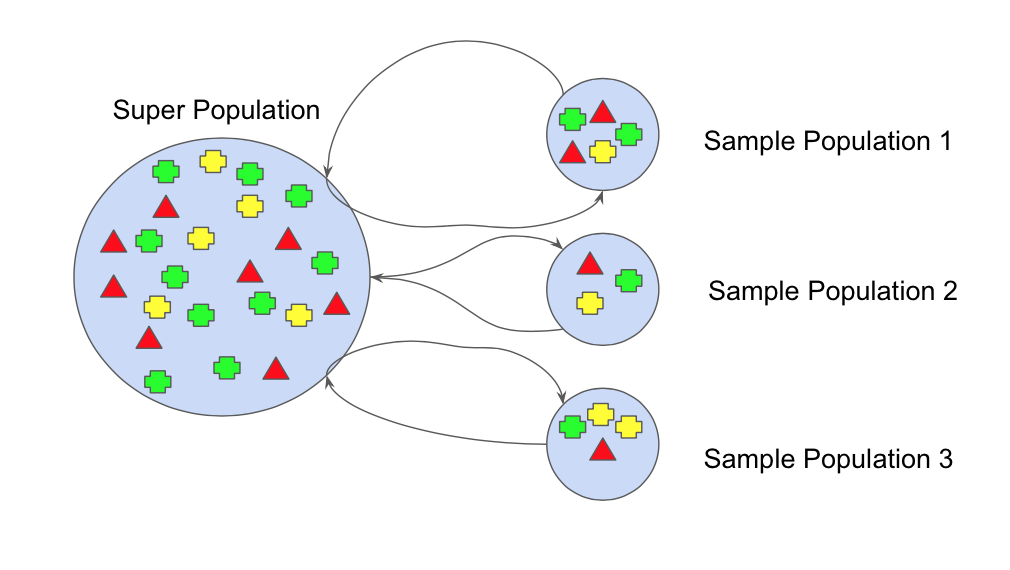
\includegraphics[width=0.7\textwidth, keepaspectratio]{imaxes/Bootstrapping.png}
    \caption[Ejemplo de \textit{Bootstrapping}]{Ejemplo de \textit{Bootstrapping}~\cite{Bootstrapping}}
    \label{fig:bootstrapping}
\end{figure}


\subsubsection{\textit{Bagging}~\cite{breiman1996bagging}}

Este método genera  múltiples instancias de un mismo modelo predictivo para conseguir una mejora en la precisión de la predicción. Generalmente esta técnica puede ser usada para reducir en algoritmos que tienen una alta varianza para reducirla.


\subsubsection{\textit{Boosting}}
Esta técnica emplea un conjunto de algoritmos que utilizan promedios ponderados para convertir aprendizajes débiles en fuertes. Cada modelo ejecutado, dicta en que características se centrará el siguiente modelo.

\begin{figure}[h]
    \centering
    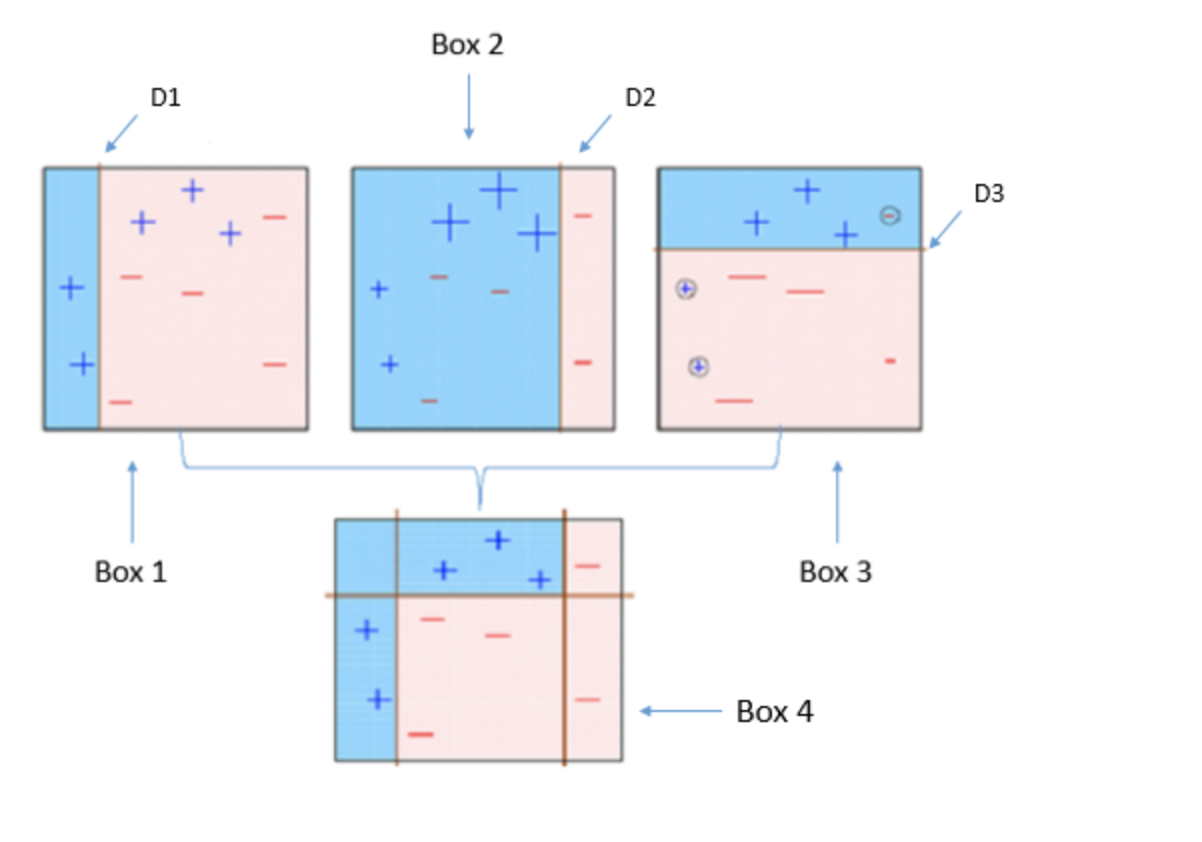
\includegraphics[width=0.7\textwidth, keepaspectratio]{imaxes/boosting.png}
    \caption[Ejemplo de \textit{Boosting}]{Ejemplo de \textit{Boosting}~\cite{bossting}}
    \label{fig:bossting}
\end{figure}

\subsubsection{\textit{Stacking}}
Esta técnica combina múltiples modelos de clasificación o regresión. Los modelos son entrenados individualmente utilizando un conjunto de entrenamiento y sus resultados son combinados para obtener una predicción final.

\subsection{Bosques Aleatorios}
\label{sec:random_forest}
Los bosques aleatorios~\cite{Breiman2001} también conocidos como \textit{Random Forest}, fueron desarrollados por \textbf{Leo Breiman} y \textbf{Adele Cutler}. Este algoritmo utiliza la técnica de \textit{Bagging} para realizar las predicciones.

Son un conjunto de árboles de decisión en el que cada árbol depende de los valores de un vector aleatorio probado independientemente y con la misma distribución para cada uno de los árboles del bosque [Figura~\ref{fig:schematic_RandomForest}].




\subsubsection{Ventajas}

Las ventajas de los \textit{Random Forest} son:

\begin{itemize}
    \item Es uno de los algoritmos de aprendizaje más fiables.
    \item Funciona bien con conjunto de datos muy grandes.
    \item Puede manejar cientos de variables de entrada.
    \item Guarda la información sobre las variables más importantes.
\end{itemize}

\subsubsection{Desventajas}

\begin{itemize}
    \item No funcionan bien cuando hay variables categóricas.
    \item Puede sobre ajustar en ciertos grupos de datos con mucho ruido.
\end{itemize}



\begin{figure}[h]
    \centering
    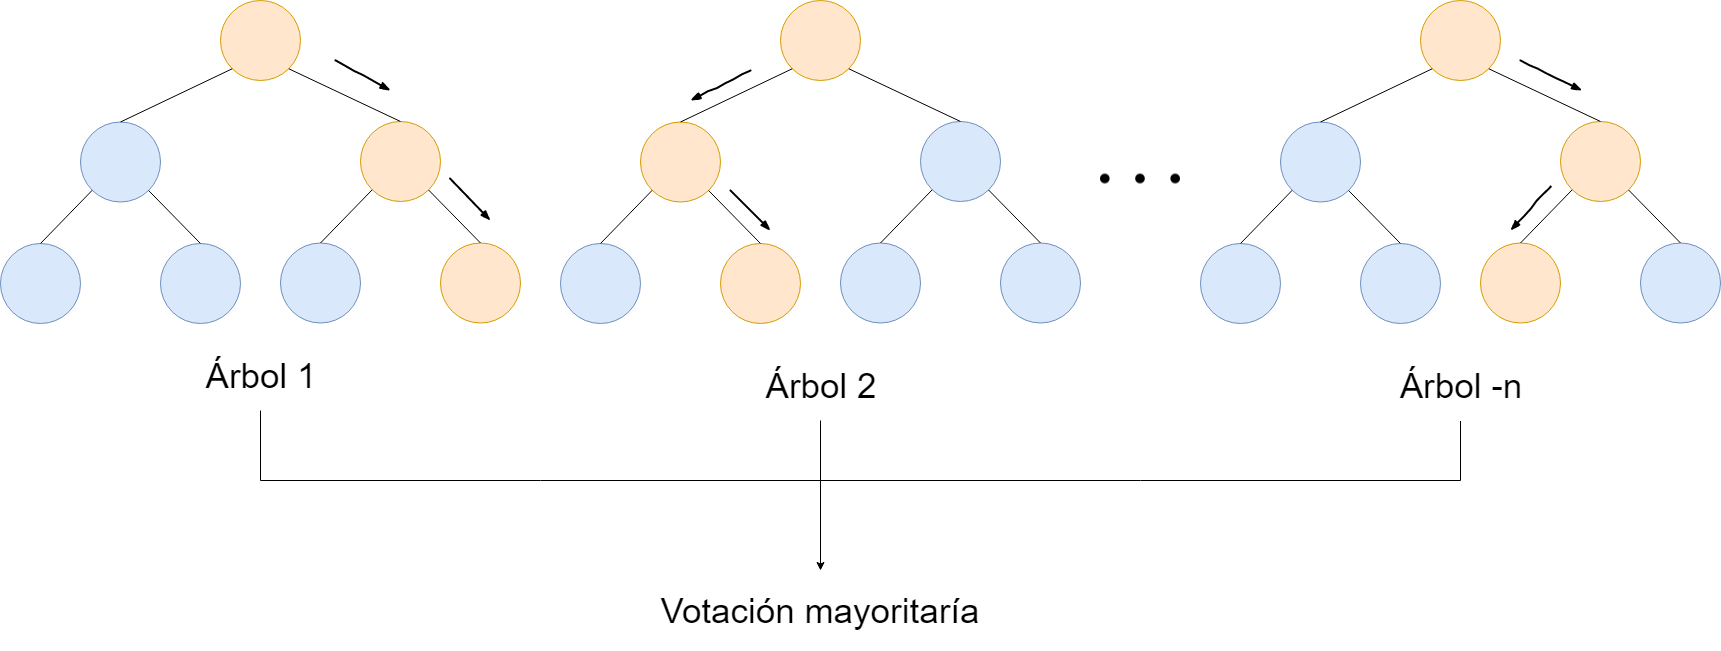
\includegraphics[width=0.9\textwidth, keepaspectratio]{imaxes/random_forest.png}
    \caption{Esquema \textit{Random Forest}}
    \label{fig:schematic_RandomForest}
\end{figure}



% ======================================================== %

% ======================================================== %


\subsection{Clasificador por Votación} 
\label{sec:voting_clf}

La clasificación por votación~\cite{voting_clf} es un meta-clasificador, es decir, no implementa un algoritmo de clasificación sino que evalúa las predicciones de otros algoritmos para obtener una nueva [Figura~\ref{fig:schematic_Voting}]. Este algoritmo se basa en la técnica de \textit{Stacking} para obtener las predicciones.

\subsubsection{Tipos de votación}

\begin{itemize}
    \item \textbf{Votación Dura/Mayoritaria} :  Es un caso de selección por mayoría simple. La predicción se hace en base al mayor número de votos por parte de los algoritmos utilizados.
    
    \item \textbf{Votación Blanda} : Esta técnica calcula el mejor resultado obteniendo la media de las probabilidades calculadas por los algoritmos individualmente.
\end{itemize}

\subsubsection{Ventajas}

\begin{itemize}
    \item Por norma general suelen proporcionar mejores resultados, si se rigen por ciertas condiciones, como que los clasificadores sean totalmente independientes~\cite{RUTA200563}.
\end{itemize}

\subsubsection{Desventajas}

\begin{itemize}
    \item No todos los algoritmos son válidos para esta técnica, especialmente cuando se usa el método de votación blanda, ya que no todos los algoritmos estiman las probabilidades de las salidas.
\end{itemize}


\begin{figure}[h]
    \centering
    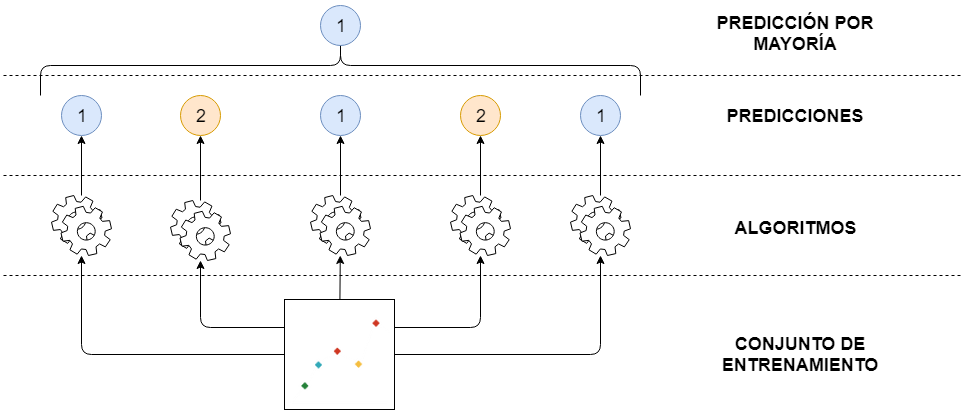
\includegraphics[width=1\textwidth, keepaspectratio]{imaxes/schema_voting.png}
    \caption{Esquema clasificación por votación}
    \label{fig:schematic_Voting}
\end{figure}
